%% DESIGN: Charter + Helvetica | Two-column academic-modern hybrid | Dark purple (#4B0082) accent
\documentclass[11pt,a4paper]{article}
\usepackage[left=0.7in,right=0.7in,top=0.6in,bottom=0.6in]{geometry}
\usepackage[T1]{fontenc}
\usepackage{charter}
\usepackage[scaled=0.92]{helvet}
\usepackage{xcolor,titlesec,enumitem,hyperref,multicol,fancyhdr}
\usepackage{tikz}

\definecolor{accent}{HTML}{4B0082}
\definecolor{ACCENT}{HTML}{4B0082}
\hypersetup{colorlinks=true,linkcolor=accent,urlcolor=accent}
\pagestyle{empty}

\titleformat{\section}{\large\bfseries\sffamily\color{accent}}{}{0em}{}[\vspace{-0.5em}\textcolor{accent}{\rule{\linewidth}{1.2pt}}]
\titlespacing{\section}{0pt}{1em}{0.5em}

\newcommand{\entry}[4]{\noindent\textbf{#1} \hfill \textit{#2}\\#3 \hfill #4\vspace{0.4em}}

\begin{document}

% Header
\begin{center}
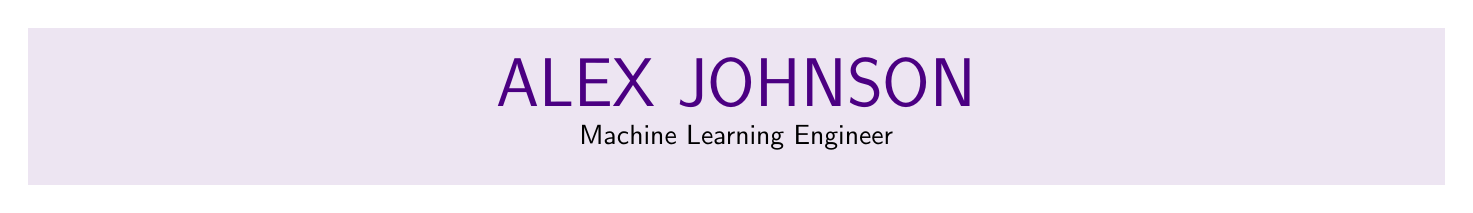
\begin{tikzpicture}
\fill[accent!10] (-9,-0.8) rectangle (9,1.2);
\node at (0,0.5) {\Huge\bfseries\sffamily\color{accent} ALEX JOHNSON};
\node at (0,-0.2) {\sffamily Machine Learning Engineer};
\end{tikzpicture}
\end{center}
\vspace{-0.5em}
\begin{center}
\small alex.johnson@email.com $\cdot$ (555) 123-4567 $\cdot$ San Francisco, CA $\cdot$ \href{https://linkedin.com/in/alexjohnson}{LinkedIn} $\cdot$ \href{https://github.com/alexj}{GitHub}
\end{center}

\vspace{0.5em}

\begin{multicols}{2}
\section{Summary}
ML Engineer with 5+ years building production ML systems. Published researcher with expertise in deep learning, NLP, and scalable model deployment. Passionate about bridging research and industry applications.

\section{Publications}
\begin{itemize}[leftmargin=*,nosep,label={\color{accent}$\blacktriangleright$}]
\item \textbf{Johnson, A.} et al. ``Efficient Transformer Pruning for Edge Deployment,'' \textit{NeurIPS 2024}.
\item \textbf{Johnson, A.}, Smith, B. ``Federated Learning at Scale,'' \textit{ICML 2023}.
\end{itemize}

\columnbreak

\section{Technical Skills}
\begin{description}[style=nextline,font=\sffamily\color{accent},nosep]
\item[ML/DL] PyTorch, TensorFlow, JAX, Hugging Face
\item[Infrastructure] Kubernetes, Docker, AWS SageMaker
\item[Languages] Python, C++, Rust, SQL
\item[Methods] Transformers, GNNs, RL, Bayesian Methods
\end{description}
\end{multicols}

\section{Experience}
\entry{Senior ML Engineer}{Jan 2022 -- Present}{TechCorp AI, San Francisco, CA}{}
\begin{itemize}[leftmargin=1.5em,nosep,label={\color{accent}\textbullet}]
\item Designed and deployed transformer-based recommendation system serving 50M+ users, improving CTR by 23\%
\item Led model optimization initiative reducing inference latency by 40\% through quantization and distillation
\item Mentored team of 4 junior ML engineers; established ML code review practices
\end{itemize}
\vspace{0.3em}

\entry{ML Engineer}{Jun 2019 -- Dec 2021}{DataDriven Inc., Mountain View, CA}{}
\begin{itemize}[leftmargin=1.5em,nosep,label={\color{accent}\textbullet}]
\item Built end-to-end ML pipeline processing 10TB+ daily data for fraud detection (precision: 0.94)
\item Implemented A/B testing framework for ML models, enabling rapid experimentation
\item Published internal research on few-shot learning applied to customer segmentation
\end{itemize}

\section{Education}
\entry{M.S. Computer Science (Machine Learning)}{2017 -- 2019}{Stanford University}{}
\entry{B.S. Mathematics \& Computer Science}{2013 -- 2017}{UC Berkeley}{}

\section{Awards}
\begin{itemize}[leftmargin=1.5em,nosep,label={\color{accent}\textbullet}]
\item Best Paper Award, Internal ML Conference 2023
\item Patent: ``Adaptive Model Serving Architecture'' (US Patent Pending)
\end{itemize}

\end{document}
